\documentclass[a4paper,11pt]{article}

\usepackage[english]{babel}
\usepackage{amsmath,amssymb,amsthm}
\usepackage{hyperref}
\usepackage{graphicx}

\newtheorem{prop}{Proposition}
\DeclareMathOperator{\Arg}{Arg} % This line defines \Arg

% Please don't change the settings above. 
% Don't change margins, fonts (including size) or make any other alterations which would either expand or contract the length of the resulting file. 
% You can add packages if you need but these should not impact on the length of the document, the markers have discretion to determine if such additions are appropriate. You should not need to add any packages for the first assignment.


\title{HCoV Skill Assignment 2}
\author{Harry Han, S2162783}

\begin{document}
\maketitle

% Format each task below in a new section with an appropriate heading.

% 1. Put an appropriate section heading here.
\section{Hutton's Proof Without Word Explained}

% Replace this paragraph based on your solution to Exercise~2.3 from Workshop 2, explaining why the figure establishes the identity

Equation \ref{eq:triangle} is daunting at the first glance.
Very few elementary algebraic properties are left in our repertoire to handle the constant $\pi$ and the inverse trigonometry functions, the capricious gnomes that only shine with the glamour of higher mathematics.

Yet Hutton had provided us a genius and intuitive proof with figure \ref{fig:Hutton's_Proof}.
To further convince you with rhetoric, dear reader, may you notice $\frac{\pi}{4} = \angle BAE = \angle BAC + \angle CAD + \angle DAE$.
By carefully counting the grids we find $AE$ is seven times the length of $DE$, $AC$ is thrice of $BC$, and $BC$ the same as $CD$.
It is not hard to notice also that $\angle BCD = \angle ACD = \angle DEA = \frac{\pi }{2}$. In this way, after recalling the definition of $\arctan$ function, that is, it returns the angle from the ratio of the opposite side and the adjacent side, the grandeur of equation \ref{eq:triangle} is complete.

\begin{equation}\label{eq:triangle}
	\dfrac{\pi}{4} = 2\arctan\left( \frac{1}{3} \right) + \arctan \left( \frac{1}{7} \right).
\end{equation}

\begin{figure}[htbp]
	\centering
	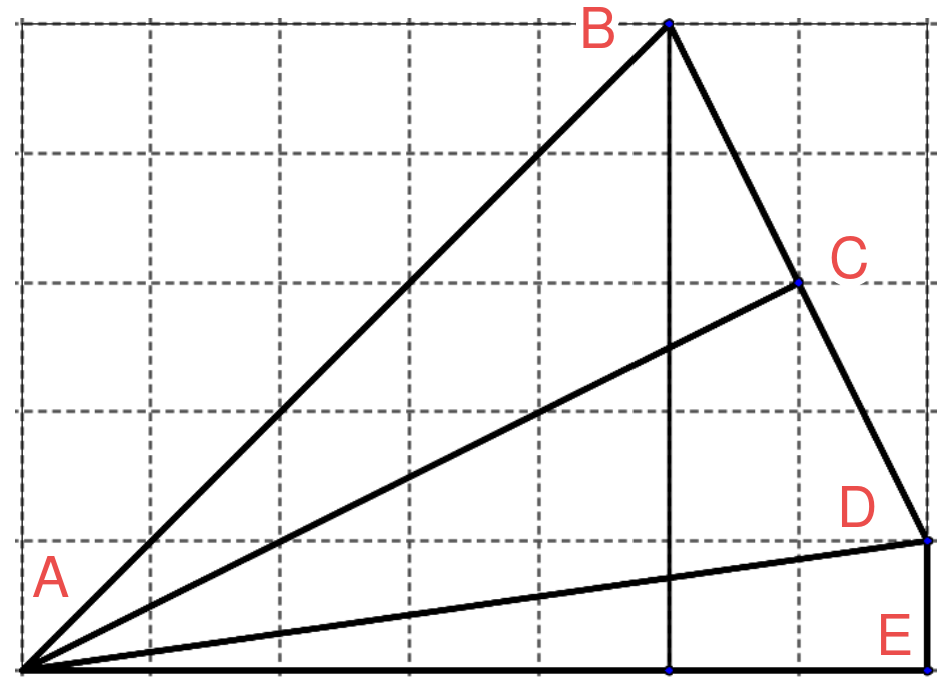
\includegraphics[width=0.6\textwidth]{./hutton.png}
	\caption{Hutton's Proof for Equation \ref{eq:triangle}.}
	\label{fig:Hutton's_Proof}
\end{figure}

\section*{Exercise 2.5: Arguments of Complex Number}

Any complex number $z$ can be written in the exponential form $z = |z|e^{i\theta}$, where $|z|$ is the norm of $z$ and $\theta$, intuitively speaking, the angle $z$ makes with the $x$ axis.
Notice that adding any multiple of $2\pi$ to $\theta$ will not change its value. Thus, we define the set of all possible value of $\theta$ to be $\arg(z)$. If we further restrict $-\pi<\theta \leq \pi$, it is the principle argument of $z$ and denoted as $\Arg(z)$. Note that $\arg(z) = \{\Arg(z) + 2k\pi : k \in \mathbb{Z}\}$.

\section*{Exercise 2.8: Real Valued Holomorphic Function is Constant}

\begin{prop}
	If the function $f$ is holomorphic on $\mathbb{C}$ and only takes real values (i.e., its codomain is $\mathbb{R}$), then $f$ is constant.
\end{prop}

\begin{proof}
	We are foremost behooved to explain our interpretation for the verb ``take''.
	The ambiguity lies on its mood: if it is intended to be used in active mood, ``take real value'' means the domain of the function is real; or, used in passive mood, it means the co-domain is real. The former connotation, I proclaim, is not plausible, as it is impossible to find a neighborhood on $\mathbb{C}$ that only contains real number, leading to the consequence that non of the functions with only real domain would be holomorphic.

	After realizing this fact the proof becomes a trivial adaptation of the Cauchy-Riemann equations. 
	For any $z = x + iy$, the function $f$, whose codomain is $\mathbb{R}$, can be written as $f(z) = u$, where $u \in \mathbb{R}$.
	Apply Cauchy-Riemann equation, we can find, for all $x, y$ in its domain: 
	\begin{equation}\label{eq:cauchy_riemann}
		\frac{\partial u}{\partial x} = \frac{\partial u}{\partial y} = 0
	\end{equation}
	I will convince you that it is a sufficient condition for $f$ to be constant.
	For, if, for certain $z_1 = x_1+iy_1, z_2 = x_2+iy_2$, $f(x_1 + iy_1) \neq f(x_2 + iy_2)$, as $f$ is holomorphic, we can invoke mean value theorem to see that there exist a point in certain curve connecting $x_1 + iy_1$ and $x_2+iy_2$ such that its gradient is non-zero, contradicting equation \ref{eq:cauchy_riemann}.
\end{proof}

\end{document}
